%
% $RCSfile: domain_model.tex,v $
%
% Copyright (C) 2002-2008. Christian Heller.
%
% Permission is granted to copy, distribute and/or modify this document
% under the terms of the GNU Free Documentation License, Version 1.1 or
% any later version published by the Free Software Foundation; with no
% Invariant Sections, with no Front-Cover Texts and with no Back-Cover
% Texts. A copy of the license is included in the section entitled
% "GNU Free Documentation License".
%
% http://www.cybop.net
% - Cybernetics Oriented Programming -
%
% http://www.resmedicinae.org
% - Information in Medicine -
%
% Version: $Revision: 1.1 $ $Date: 2008-08-19 20:41:06 $ $Author: christian $
% Authors: Christian Heller <christian.heller@tuxtax.de>
%

\subsubsection{Domain Model}
\label{domain_model_heading}
\index{Domain Model Pattern}

One of the three layers in figure \ref{logical_figure} shown at the beginning
of this chapter is the \emph{Domain Model}. Fowler \cite{fowler2002} proposed
it as singular pattern because of its importance in large-scale business
systems. Figure \ref{domainmodel_figure} shows an imaginary business domain
model. The actual focus, however, should not be put on the inside structure of
this example model, but on the fact that the domain model represents a layer on
its own.

\begin{figure}[ht]
    \begin{center}
        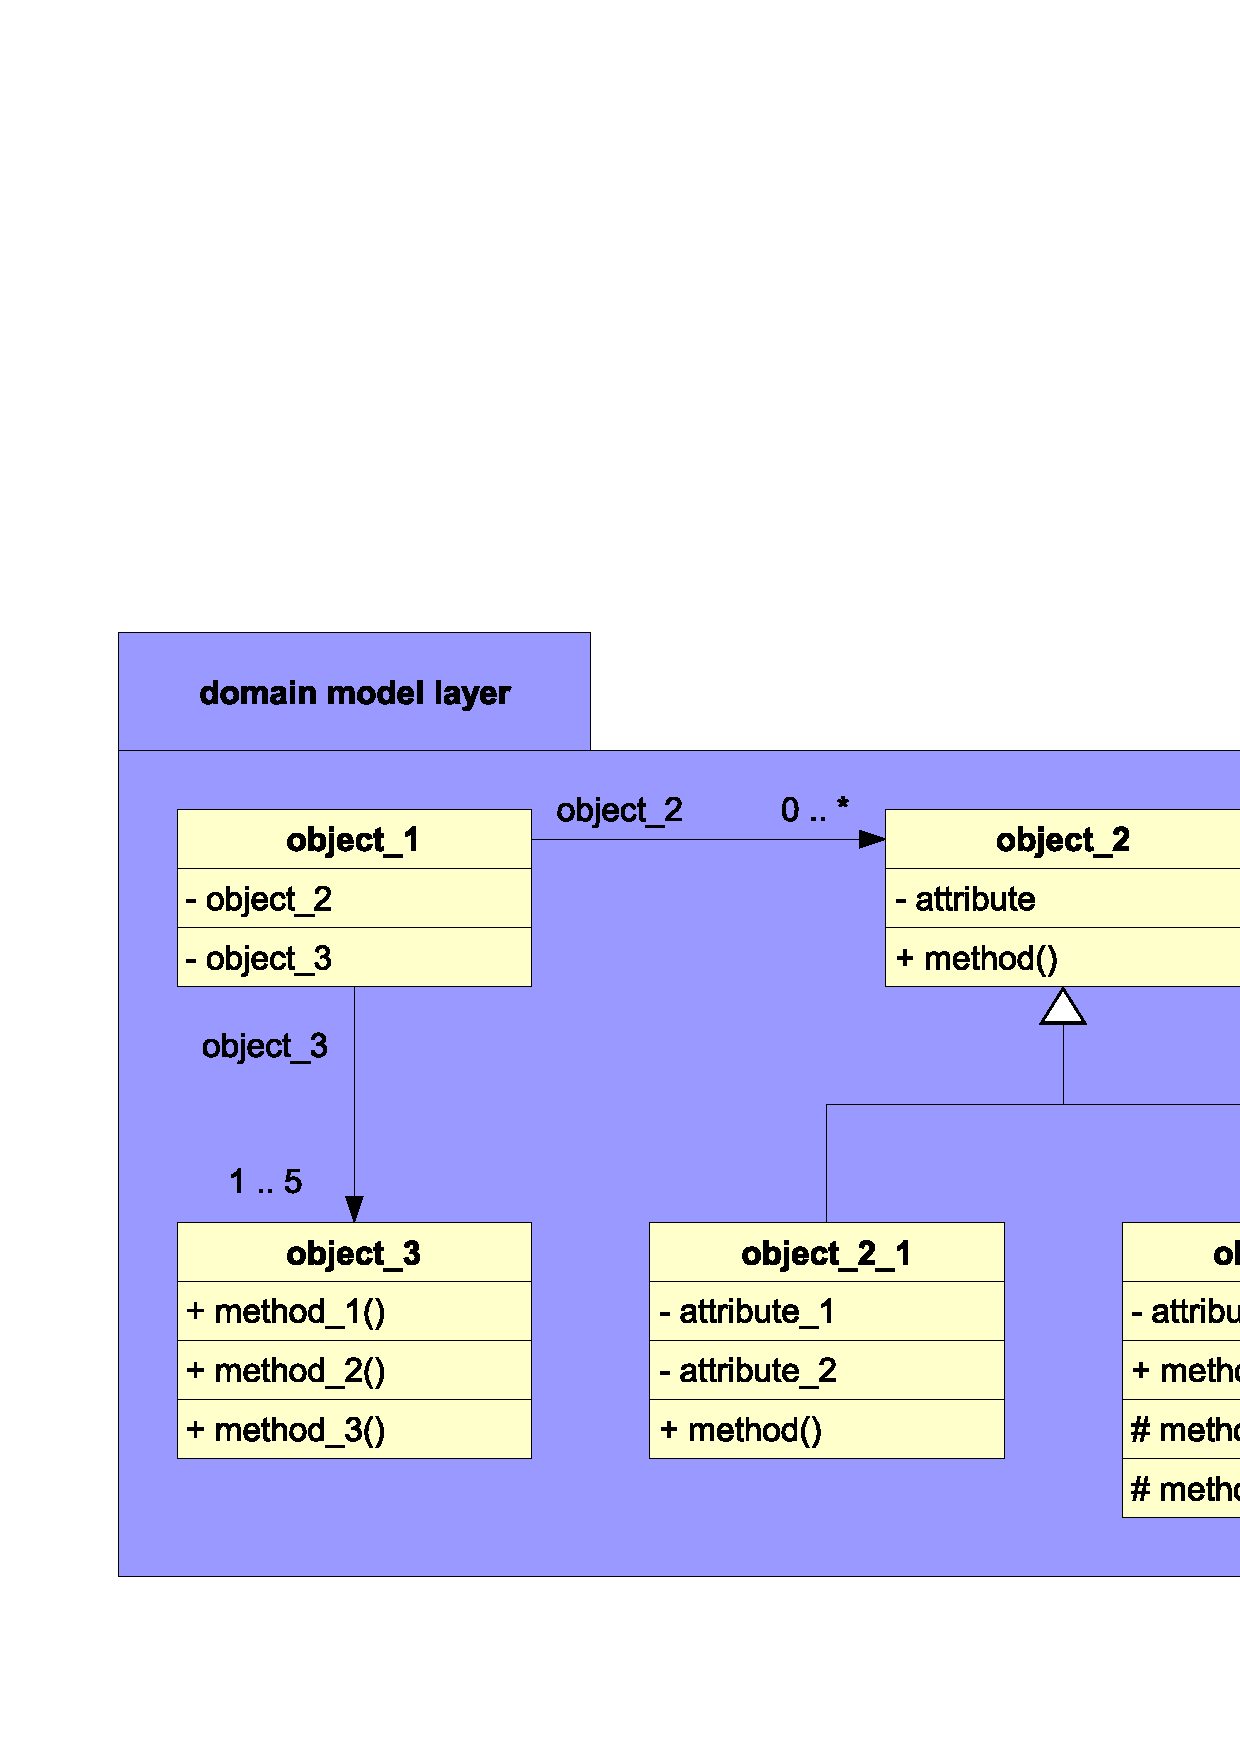
\includegraphics[scale=0.3,angle=-90]{graphic/domainmodel.pdf}
        \caption{Domain Model Pattern}
        \label{domainmodel_figure}
    \end{center}
\end{figure}

This separation cannot be found in all systems and in fact, it does not make
sense for \emph{all} systems. Small solutions let their user interface or
application control, respectively, access a database directly which avoids the
rather big effort of creating a special domain model. But the larger the system
to be created and the more clear the desired architecture shall be, the more
recommendable it is to use the \emph{Domain Model} pattern.

It will be helpful to have heard about this pattern when reading chapter
\ref{state_and_logic_heading} dealing with domain-, user interface- and other
models and their translation into each other.
